\documentclass[UTF8,ctexart,a4paper,11pt,openany]{article}
\usepackage[slantfont,boldfont]{xeCJK}
\usepackage{fontspec}
\usepackage{ctex}
\usepackage{booktabs}
\setCJKmainfont{SimSun}%[BoldFont=SimHei] %去掉注释:bf字体为黑体

\setsansfont{SimHei}
\setCJKsansfont{SimHei}

\xeCJKsetcharclass{"2160}{"2470}{1}% 1: CJK
\xeCJKsetup{AutoFallBack=true}
\setCJKfallbackfamilyfont{\CJKrmdefault}{SimSun.ttf}

%\setmainfont{Times New Roman}     %去掉注释:Times new roman字体
%\usepackage{mathptmx}             %去掉注释:Times new roman字体

\usepackage{mathtools}
\usepackage{amsmath}
\usepackage{amsfonts}
\usepackage{amssymb}
\usepackage{amsthm}
\usepackage[T1]{fontenc}
\usepackage{indentfirst} %段首空两格

\usepackage{graphicx}
\usepackage{geometry}
\usepackage{latexsym}
\usepackage{fancyhdr}
\usepackage{epstopdf}
%\usepackage{pifont}
%\usepackage[perpage,symbol*]{footmisc}
\usepackage{titlesec}
\usepackage{setspace}
\usepackage{enumerate}
\usepackage{enumitem}
\usepackage{multicol}
\usepackage{url}
\usepackage{exscale}
\usepackage{ulem}
\usepackage{relsize}
\usepackage{mathrsfs}
\usepackage{tikz}
\usepackage{wrapfig}
\usepackage{framed}
\usepackage{bm}
%\usepackage{pstricks,pst-node,multido,ifthen,calc}
\usepackage[all]{xy}
\usepackage{extarrows}
%\usepackage[backref]{hyperref}
\usepackage{hyperref}
\usepackage{stfloats} %插图的时候不分页

\setlength{\parindent}{2em} %段首空两格
\linespread{1.2}
\usepackage{listings}
\usepackage{xcolor}
\usepackage{algorithm}
\usepackage{algorithmicx}
\usepackage{algpseudocode}
\usepackage{mdframed}
\usepackage{extarrows}
\usepackage{diagbox}
\usepackage{makecell}

\theoremstyle{definition}
\mdfdefinestyle{theoremstyle}{%
linecolor=green!40,linewidth=.5pt,%
backgroundcolor=green!10,
skipabove=8pt,
skipbelow=5pt,
innerleftmargin=7pt,
innerrightmargin=7pt,
frametitlerule=true,%
frametitlerulewidth=.5pt,
frametitlebackgroundcolor=green!35,
frametitleaboveskip=0pt,
frametitlebelowskip=0pt,
innertopmargin=.4\baselineskip,
innerbottommargin=.4\baselineskip,
shadow=true,shadowsize=3pt,shadowcolor=black!20,
%theoremseparator={\hspace{1pt}},
theoremseparator={.},
nobreak=true,
}


\everymath{\displaystyle}

\newtheorem{definition}{\hspace{2em}定义}[section]
\newtheorem{axiom}{\hspace{2em}公理}

\mdtheorem[style=theoremstyle]{theorem}{定理}
\mdtheorem[style=theoremstyle]{example}{例}
\mdtheorem[style=theoremstyle]{exercise}{问题}
\newtheorem{lemma}[theorem]{\hspace{2em}引理}
\newtheorem{corollary}[theorem]{\hspace{2em}推论}

\newcommand*{\QED}{\hfill\ensuremath{\square}}
\newcommand*{\rmk}{\textbf{注:}}
\renewcommand*{\proof}{\textbf{证明:}}
\newcommand*{\tips}{\textbf{提示:}}
\newcommand*{\hard}{\textbf{\color{red}(难)}}
\newcommand*{\eqsmall}{\setlength\abovedisplayskip{1pt}\setlength\belowdisplayskip{1pt}}
\geometry{left=2cm,right=2cm,top=2cm,bottom=2cm}
% \title{数值分析上机报告(示例}
% \author{Fiddie}
\pagestyle{fancy}
\fancyfoot[C]{}
\fancyhead[RO]{ \thepage}
\fancyhead[LE]{\thepage  }
% \fancyhead[RE]{\rightmark (By Fiddie)}
% \fancyhead[LO]{\leftmark (By Fiddie)}
\titleformat{\chapter}{\centering\huge\bfseries}{第\,\thechapter\,章}{1em}{} %更改标题样式
\titleformat{\section}{\bfseries\Large}{$\S$\,\thesection\,}{1em}{} %更改标题样式
\titlespacing*{\chapter}{0pt}{9pt}{0pt} %调整标题间距
\setenumerate[1]{itemsep=0pt,partopsep=0pt,parsep=\parskip,topsep=0pt} %设置enumerate行间距
\setenumerate[2]{itemsep=0pt,partopsep=0pt,parsep=\parskip,topsep=0pt} %设置enumerate行间距
\setitemize[1]{itemsep=0pt,partopsep=0pt,parsep=\parskip,topsep=0pt} % 设置itemize行间距
\setlist[enumerate,2]{label=(\arabic*),topsep=0mm,itemsep=0mm,partopsep=0mm,parsep=\parskip}
% 设置二层枚举为(1)样式
    
\newfontfamily\hei{SimHei}
\newcommand\textcf[1]{\textbf{\textsf{\hei{#1}}}}

\newcommand\e{\leftarrow}
%\renewcommand{\bibname}{参考文献}

\begin{document}
\begin{center}
{\huge \textbf{《数值分析》上机期末考试报告}}

{\large 学号:221840189,姓名:王晨光}
\end{center}

\section{问题}
    应用 Runge-Kutta-Fehlberg 算法解初值问题:$$\begin{aligned}
        y' =  -y&+t^2+2, \quad 0\le t\le 1, \\
        y(0) = & 1
    \end{aligned}$$
    取$TOL=10^{-4}$, $h_{\text{max}}=0.2$, $h_{\text{min}}=0.0001$.\par 分别用表和图给出计算结果. 
\section{算法思路}
    在微分方程数值解法中,步长$h$ 的选择是很重要的.但是,要做到合理选择也 
    是比较困难的,因为它与问题本身和所选用的数值方法都有关系.前面介绍的 
    Runge-Kutta方法,实际上,往往并不直接应用它们.一 般地,使用者要求数值解与 
    精确解之差不超过某一误差容限.由这个容限来确定数值方法中应取多大的步长. 
    为了选取比较合适的步长,一方面必须对局部(每一步)误差有一个估计;另一方面 
    在整个区间不取固定的步长$h$,在区间的某些段上取相对小的$h$,而在另一些段上 
    则取相当大的$h$. \par
    以三阶 Runge-Kutta 方法为例,记$$\tau_{n+1}=(y(t_{n+1})-y_{n+1})/h$$则存在常数$K$使得$$\tau _{n+1}\backsimeq Kh^2$$可以写成$$Kh^2\backsimeq \frac{1}{h}(u_{n+1}-y_{n+1})$$由给定的误差容限度$TOL$,我们可以选取$q$使得:$$q\leqslant \left[\frac{TOL}{\frac{|u_{n+1}-y_{n+1}|}{h}}\right]^{\frac{1}{2}}$$假定$u_n=y_n$可以得到:$$\frac{u_{n+1}-y_{n+1}}{h}=\frac{2K_1+4K_3-6K_2}{9}$$\indent 若$$\frac{\left|u_{n+1}-y_{n+1}\right|}{h}\leqslant TOL$$则取$q=1$,且下一步仍然使用$h$;若:$$\frac{\left|u_{n+1}-y_{n+1}\right|}{h}> TOL$$则将步长缩小,重新计算为了确保步长缩小不至无限循环下去,我们给出一个步长的下限,如$h_{\text{min}}$. 若$h<h_{\text{min}}$,则终止计算;若$\frac{\left|u_{n+1}-y_{n+1}\right|}{h}$比$TOL$小到一定程度,则增大步长. \par
    Fehlberg 于 1970 年提出用五阶 Runge-Kutta 方法:$$u_{n+1}=u_n+\frac{16}{135}K_1+\frac{6656}{12825}K_3+\frac{28561}{56430}K_4-\frac{9}{50}K_5+\frac{2}{55}K_6$$去估计四阶 Runge-Kutta 方法:$$y_{n+1}=y_n+\frac{25}{216}+\frac{1408}{2565}K_3+\frac{2197}{4104}K_4-\frac{1}{5}K_5$$其中:$$    \left\{\begin{array}{l}
        K_{1}=hf\left(t_{n}, y_{n}\right) \\ 
        K_{2}=hf\left(t_{n}+\frac{h}{4}, y_{n}+\frac{1}{4}K_1\right) \\ 
        K_{3}=hf\left(t_{n}+\frac{3}{8}h, y_{n}+\frac{3}{32}K_1+\frac{9}{32}K_2\right) \\ 
        K_{4}=hf\left(t_{n}+\frac{12}{12}h, y_{n}+\frac{1932}{2197}K_1-\frac{7200}{2197}K_2+\frac{7296}{2197}K_3\right) \\ 
        K_{5}=hf\left(t_{n}+h, y_{n}+\frac{439}{216}K_1-8K_2+\frac{3680}{513}K_3-\frac{845}{4104}K_4\right) \\ 
        K_{6}=hf\left(t_{n}+\frac{h}{2}, y_{n}-\frac{8}{27}K_1+2K_2-\frac{3544}{2565}K_3+\frac{1859}{4104}K_4-\frac{11}{40}K_5\right)  
    \end{array}
    \right.$$我们称它为 \textbf{Runge-Kutta-Fehlberg} 方法,简称 \textbf{R-K-F} 方法. 显然,这个方法的优点
    是每一步只要计算6个函数值. 而其他四阶和五阶 Runge-Kutta 方法一起使用时, 
    每一步将要求计算10个函数值. \par
    由于两式的局部离散误差分别为$O(h^6)$和$O(h^5)$,因此我们有:$$\tau _{n+1}\backsimeq Kh^4$$和$$Kh^4\backsimeq\frac{1}{h}(u_{n+1}-y_{n+1})$$从而得到了:$$q\leqslant \left[\frac{TOL}{\frac{|u_{n+1}-y_{n+1}|}{h}}\right]^{\frac{1}{4}}$$实际使用时,通常取$$q=\left[\frac{TOL}{\frac{2|u_{n+1}-y_{n+1}|}{h}}\right]^{\frac{1}{4}}=0.84\left[\frac{TOL}{\frac{|u_{n+1}-y_{n+1}|}{h}}\right]^{\frac{1}{4}}$$现在进一步修改得到:$$\frac{|u_{n+1}-y_{n+1}|}{h}=\left|\frac{1}{360}K_1-\frac{128}{4275}K_3-\frac{2197}{75240}K_4+\frac{1}{50}K_5+\frac{2}{55}K_6\right|/h$$\indent 此后继续沿用上述的自适应法则. 
    \begin{algorithm}[H]
        \caption{\textbf{Runge-Kutta-Fehlberg} 方法}
        \begin{algorithmic}[1] %每行显示行号
            \Require 区间$[a,b]$; 初值$\eta $; 积分函数$f$; 最大步长$h_{max}$; 最小步长$h_{min}$; 误差容限$TOL$.
            \Ensure $t$, $y$, 步长$h$
            \Function {Runge-Kutta-Fehlberg}{$a,b,\eta,f, h_{max}, h_{min}, TOL$}
                \State $t \e a$
                \State $y\e \eta$
                \State $h\e h_{max}$
                \For {$t<b$}
                    \State $K_1\e hf\left(t, y\right)$
                    \State $K_2\e hf\left(t+\frac{h}{4}, y+\frac{1}{4}K_1\right)$
                    \State $K_3\e hf\left(t+\frac{3}{8}h, y+\frac{3}{32}K_1+\frac{9}{32}K_2\right)$
                    \State $K_4\e hf\left(t+\frac{12}{12}h, y+\frac{1932}{2197}K_1-\frac{7200}{2197}K_2+\frac{7296}{2197}K_3\right)$
                    \State $K_5\e hf\left(t+h, y+\frac{439}{216}K_1-8K_2+\frac{3680}{513}K_3-\frac{845}{4104}K_4\right)$
                    \State $K_6\e hf\left(t+\frac{h}{2}, y-\frac{8}{27}K_1+2K_2-\frac{3544}{2565}K_3+\frac{1859}{4104}K_4-\frac{11}{40}K_5\right)$
                    \State $R\e \left|\frac{1}{360}K_1-\frac{128}{4275}K_3-\frac{2197}{75240}K_4+\frac{1}{50}K_5+\frac{2}{55}K_6\right|/h$
                    \State $\delta \e 0.84(TOL/R)^{\frac{1}{4}}$
                    \If {$R\leqslant TOL$}
                        \State $t\e t+h$
                        \State $y\e y+\frac{25}{216}+\frac{1408}{2565}K_3+\frac{2197}{4104}K_4-\frac{1}{5}K_5$
                        \State 输出$t,y,h$
                    \EndIf
                    \If {$\delta \leqslant 0.1$}
                        \State $h\e 0.1h$
                    \Else
                        \If {$\delta \geqslant4$}
                            \State $h\e 4h$
                        \Else 
                            \State $h\e \delta h$
                        \EndIf
                    \EndIf 
                    \If {$h\geqslant h_{max}$}
                        \State $h\e h_{max}$
                    \EndIf
                    \If {$h< h_{min}$}
                        \State break
                    \EndIf 
                \EndFor
            \EndFunction
        \end{algorithmic}
    \end{algorithm}
\section{结果分析}
    我们将使用 python 中 scipy 库中的integrate.solve\_ivp函数求解得到的结果作为该初值问题的精确解,并与通过\textbf{R-K-F}方法得到的结果进行比较. \par
    \begin{figure}[H]
        \centering
        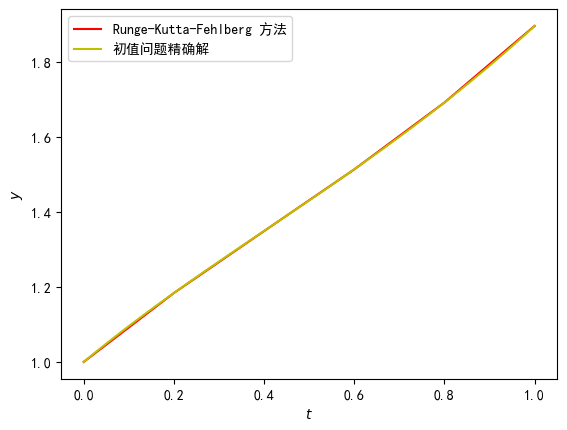
\includegraphics[width=0.6\linewidth]{pics/exam.png}
        \caption{使用\textbf{R-K-F}方法得到的结果与精确结果的比较图}
    \end{figure}
    \begin{table}[H]
        \centering
        % \resizebox{\textwidth}{!}{%
        \begin{tabular}{ccc} % 注明列数
            \toprule
            $t$   & $y$                   & Runge-Kutta-Fehlberg        \\ \midrule
            0 & 1.0 & 1 \\
            0.2 & 1.1838953507690455 & 1.1838083076923076 \\
            0.4 & 1.3493627038060534 & 1.3490406228872582 \\
            0.6000000000000001 & 1.5137912922810752 & 1.5135657904689523 \\
            0.8 & 1.6919546132170773 & 1.6920135743911044 \\
            1.0 & 1.896184383974114 & 1.896361805046761\\ \bottomrule
        \end{tabular}
        %}
        \caption{使用\textbf{R-K-F}方法得到的结果与精确结果的比较表}
    \end{table}
    \indent 从图、表中可以看出,\textbf{R-K-F}方法用于求解该微分方程初值问题有非常精确的效果. 
\section{结论}
    \textbf{Runge-Kutta-Fehlberg} 方法巧妙地将“自适应”的思想引入到微分方程数值解的经典方法五阶 \textbf{Runge-Kutta} 方法中,有着很不俗的表现. 可以被我们广泛地用于求微分方程的精确数值解. 
\clearpage

\section{附录: 程序代码}
\lstset{
    numbers=left,
    language=Python,
    keywordstyle=\color{blue!100},
    commentstyle=\color{green!50!blue!50!},
    frame=shadowbox,%阴影
    escapeinside='',%英文分号输入中文
    xleftmargin=2em,xrightmargin=2em,aboveskip=1em,
    framexleftmargin=2em,
    extendedchars=false}
\begin{lstlisting}[aboveskip=0pt]
import numpy as np
import matplotlib.pyplot as plt
plt.rcParams['font.sans-serif'] = ['SimHei']
plt.rcParams['axes.unicode_minus'] = False
# 初始条件和步长
x0, y0 = 0, 1
x1 = 1
h_min = 0.0001
h_max = 0.2
tol = 1e-4
# 定义常微分方程
def f(x, y):
    return -y + x**2 + 2

def runge_kutta_4(f, x0, x1, y0, tol, hmax, hmin):
    y1=[]
    x=[]
    t = x0
    y = y0
    y1.append(y0)
    x.append(x0)
    h = hmax
    while t < x1:
        k1=h*f(t,y)
        k2=h*f(t+0.25*h,y+0.25*k1)
        k3=h*f(t+(3/8)*h,y+(3/32)*k1+(9/32)*k2)
        k4=h*f(t+(12/13)*h,y+(1932/2197)*k1-(7200/2197)*k2+(7296/2197)*k3)
        k5=h*f(t+h,y+(439/216)*k1-8*k2+(3680/513)*k3-(845/4104)*k4)
        k6=h*f(t+(1/2)*h,y-(8/27)*k1+2*k2-(3544/2565)*k3+(1859/4104)*k4-(11/40)*k5)
        R=np.abs((1/360)*k1-(128/4275)*k3-(2197/75240)*k4+(1/50)*k5+(2/55)*k6)
        delta=0.84*((tol/R)**(1/4))
        if R<=tol:
            t=t+h
            y=y+(25/216)*k1+(1408/2565)*k3+(2197/4104)*k4-(1/5)*k5
            x.append(t)
            y1.append(y)
        if delta<=0.1:
            h=0.1*h
        else:
            if delta>=4:
                h=4*h
            else:
                h=delta*h
        if h>hmax:
            h=hmax
        if h<hmin:
            print('stop')
            break
    return x, y1
x_rk4, y_rk4 = runge_kutta_4(f, x0, x1, y0, tol, h_max, h_min)
for i in range(len(y_rk4)):
    print(y_rk4[i])
    # print(sol.sol(x_rk4)[0][i])
    # print(x_rk4[i])
from scipy.integrate import solve_ivp
x_span=(0, 1)
y_0=np.array([1])
sol=solve_ivp(f, x_span, y_0, method='RK45', dense_output=True)
x_values = np.linspace(x_span[0], x_span[1], 1000)
y_values = sol.sol(x_values)
print("Solution: ", sol.sol(x_rk4)[0])
print("Runge-Kutta 4 Method:", y_rk4)
plt.plot(x_rk4, y_rk4, label='Runge-Kutta-Fehlberg 方法', color='r')
plt.plot(x_values, y_values[0], label='初值问题精确解', color='y')
plt.xlabel('$t$')
plt.ylabel('$y$')
plt.legend()
plt.show()
    
\end{lstlisting}

\end{document}